% Options for packages loaded elsewhere
\PassOptionsToPackage{unicode}{hyperref}
\PassOptionsToPackage{hyphens}{url}
\PassOptionsToPackage{dvipsnames,svgnames,x11names}{xcolor}
%
\documentclass[
  letterpaper,
  DIV=11,
  numbers=noendperiod]{scrartcl}

\usepackage{amsmath,amssymb}
\usepackage{iftex}
\ifPDFTeX
  \usepackage[T1]{fontenc}
  \usepackage[utf8]{inputenc}
  \usepackage{textcomp} % provide euro and other symbols
\else % if luatex or xetex
  \usepackage{unicode-math}
  \defaultfontfeatures{Scale=MatchLowercase}
  \defaultfontfeatures[\rmfamily]{Ligatures=TeX,Scale=1}
\fi
\usepackage{lmodern}
\ifPDFTeX\else  
    % xetex/luatex font selection
\fi
% Use upquote if available, for straight quotes in verbatim environments
\IfFileExists{upquote.sty}{\usepackage{upquote}}{}
\IfFileExists{microtype.sty}{% use microtype if available
  \usepackage[]{microtype}
  \UseMicrotypeSet[protrusion]{basicmath} % disable protrusion for tt fonts
}{}
\makeatletter
\@ifundefined{KOMAClassName}{% if non-KOMA class
  \IfFileExists{parskip.sty}{%
    \usepackage{parskip}
  }{% else
    \setlength{\parindent}{0pt}
    \setlength{\parskip}{6pt plus 2pt minus 1pt}}
}{% if KOMA class
  \KOMAoptions{parskip=half}}
\makeatother
\usepackage{xcolor}
\usepackage[top=1in,bottom=1in,left=1in,right=1in]{geometry}
\setlength{\emergencystretch}{3em} % prevent overfull lines
\setcounter{secnumdepth}{-\maxdimen} % remove section numbering
% Make \paragraph and \subparagraph free-standing
\ifx\paragraph\undefined\else
  \let\oldparagraph\paragraph
  \renewcommand{\paragraph}[1]{\oldparagraph{#1}\mbox{}}
\fi
\ifx\subparagraph\undefined\else
  \let\oldsubparagraph\subparagraph
  \renewcommand{\subparagraph}[1]{\oldsubparagraph{#1}\mbox{}}
\fi

\usepackage{color}
\usepackage{fancyvrb}
\newcommand{\VerbBar}{|}
\newcommand{\VERB}{\Verb[commandchars=\\\{\}]}
\DefineVerbatimEnvironment{Highlighting}{Verbatim}{commandchars=\\\{\}}
% Add ',fontsize=\small' for more characters per line
\usepackage{framed}
\definecolor{shadecolor}{RGB}{241,243,245}
\newenvironment{Shaded}{\begin{snugshade}}{\end{snugshade}}
\newcommand{\AlertTok}[1]{\textcolor[rgb]{0.68,0.00,0.00}{#1}}
\newcommand{\AnnotationTok}[1]{\textcolor[rgb]{0.37,0.37,0.37}{#1}}
\newcommand{\AttributeTok}[1]{\textcolor[rgb]{0.40,0.45,0.13}{#1}}
\newcommand{\BaseNTok}[1]{\textcolor[rgb]{0.68,0.00,0.00}{#1}}
\newcommand{\BuiltInTok}[1]{\textcolor[rgb]{0.00,0.23,0.31}{#1}}
\newcommand{\CharTok}[1]{\textcolor[rgb]{0.13,0.47,0.30}{#1}}
\newcommand{\CommentTok}[1]{\textcolor[rgb]{0.37,0.37,0.37}{#1}}
\newcommand{\CommentVarTok}[1]{\textcolor[rgb]{0.37,0.37,0.37}{\textit{#1}}}
\newcommand{\ConstantTok}[1]{\textcolor[rgb]{0.56,0.35,0.01}{#1}}
\newcommand{\ControlFlowTok}[1]{\textcolor[rgb]{0.00,0.23,0.31}{#1}}
\newcommand{\DataTypeTok}[1]{\textcolor[rgb]{0.68,0.00,0.00}{#1}}
\newcommand{\DecValTok}[1]{\textcolor[rgb]{0.68,0.00,0.00}{#1}}
\newcommand{\DocumentationTok}[1]{\textcolor[rgb]{0.37,0.37,0.37}{\textit{#1}}}
\newcommand{\ErrorTok}[1]{\textcolor[rgb]{0.68,0.00,0.00}{#1}}
\newcommand{\ExtensionTok}[1]{\textcolor[rgb]{0.00,0.23,0.31}{#1}}
\newcommand{\FloatTok}[1]{\textcolor[rgb]{0.68,0.00,0.00}{#1}}
\newcommand{\FunctionTok}[1]{\textcolor[rgb]{0.28,0.35,0.67}{#1}}
\newcommand{\ImportTok}[1]{\textcolor[rgb]{0.00,0.46,0.62}{#1}}
\newcommand{\InformationTok}[1]{\textcolor[rgb]{0.37,0.37,0.37}{#1}}
\newcommand{\KeywordTok}[1]{\textcolor[rgb]{0.00,0.23,0.31}{#1}}
\newcommand{\NormalTok}[1]{\textcolor[rgb]{0.00,0.23,0.31}{#1}}
\newcommand{\OperatorTok}[1]{\textcolor[rgb]{0.37,0.37,0.37}{#1}}
\newcommand{\OtherTok}[1]{\textcolor[rgb]{0.00,0.23,0.31}{#1}}
\newcommand{\PreprocessorTok}[1]{\textcolor[rgb]{0.68,0.00,0.00}{#1}}
\newcommand{\RegionMarkerTok}[1]{\textcolor[rgb]{0.00,0.23,0.31}{#1}}
\newcommand{\SpecialCharTok}[1]{\textcolor[rgb]{0.37,0.37,0.37}{#1}}
\newcommand{\SpecialStringTok}[1]{\textcolor[rgb]{0.13,0.47,0.30}{#1}}
\newcommand{\StringTok}[1]{\textcolor[rgb]{0.13,0.47,0.30}{#1}}
\newcommand{\VariableTok}[1]{\textcolor[rgb]{0.07,0.07,0.07}{#1}}
\newcommand{\VerbatimStringTok}[1]{\textcolor[rgb]{0.13,0.47,0.30}{#1}}
\newcommand{\WarningTok}[1]{\textcolor[rgb]{0.37,0.37,0.37}{\textit{#1}}}

\providecommand{\tightlist}{%
  \setlength{\itemsep}{0pt}\setlength{\parskip}{0pt}}\usepackage{longtable,booktabs,array}
\usepackage{calc} % for calculating minipage widths
% Correct order of tables after \paragraph or \subparagraph
\usepackage{etoolbox}
\makeatletter
\patchcmd\longtable{\par}{\if@noskipsec\mbox{}\fi\par}{}{}
\makeatother
% Allow footnotes in longtable head/foot
\IfFileExists{footnotehyper.sty}{\usepackage{footnotehyper}}{\usepackage{footnote}}
\makesavenoteenv{longtable}
\usepackage{graphicx}
\makeatletter
\def\maxwidth{\ifdim\Gin@nat@width>\linewidth\linewidth\else\Gin@nat@width\fi}
\def\maxheight{\ifdim\Gin@nat@height>\textheight\textheight\else\Gin@nat@height\fi}
\makeatother
% Scale images if necessary, so that they will not overflow the page
% margins by default, and it is still possible to overwrite the defaults
% using explicit options in \includegraphics[width, height, ...]{}
\setkeys{Gin}{width=\maxwidth,height=\maxheight,keepaspectratio}
% Set default figure placement to htbp
\makeatletter
\def\fps@figure{htbp}
\makeatother

\KOMAoption{captions}{tableheading}
\makeatletter
\@ifpackageloaded{tcolorbox}{}{\usepackage[skins,breakable]{tcolorbox}}
\@ifpackageloaded{fontawesome5}{}{\usepackage{fontawesome5}}
\definecolor{quarto-callout-color}{HTML}{909090}
\definecolor{quarto-callout-note-color}{HTML}{0758E5}
\definecolor{quarto-callout-important-color}{HTML}{CC1914}
\definecolor{quarto-callout-warning-color}{HTML}{EB9113}
\definecolor{quarto-callout-tip-color}{HTML}{00A047}
\definecolor{quarto-callout-caution-color}{HTML}{FC5300}
\definecolor{quarto-callout-color-frame}{HTML}{acacac}
\definecolor{quarto-callout-note-color-frame}{HTML}{4582ec}
\definecolor{quarto-callout-important-color-frame}{HTML}{d9534f}
\definecolor{quarto-callout-warning-color-frame}{HTML}{f0ad4e}
\definecolor{quarto-callout-tip-color-frame}{HTML}{02b875}
\definecolor{quarto-callout-caution-color-frame}{HTML}{fd7e14}
\makeatother
\makeatletter
\@ifpackageloaded{caption}{}{\usepackage{caption}}
\AtBeginDocument{%
\ifdefined\contentsname
  \renewcommand*\contentsname{Table of contents}
\else
  \newcommand\contentsname{Table of contents}
\fi
\ifdefined\listfigurename
  \renewcommand*\listfigurename{List of Figures}
\else
  \newcommand\listfigurename{List of Figures}
\fi
\ifdefined\listtablename
  \renewcommand*\listtablename{List of Tables}
\else
  \newcommand\listtablename{List of Tables}
\fi
\ifdefined\figurename
  \renewcommand*\figurename{Figure}
\else
  \newcommand\figurename{Figure}
\fi
\ifdefined\tablename
  \renewcommand*\tablename{Table}
\else
  \newcommand\tablename{Table}
\fi
}
\@ifpackageloaded{float}{}{\usepackage{float}}
\floatstyle{ruled}
\@ifundefined{c@chapter}{\newfloat{codelisting}{h}{lop}}{\newfloat{codelisting}{h}{lop}[chapter]}
\floatname{codelisting}{Listing}
\newcommand*\listoflistings{\listof{codelisting}{List of Listings}}
\makeatother
\makeatletter
\makeatother
\makeatletter
\@ifpackageloaded{caption}{}{\usepackage{caption}}
\@ifpackageloaded{subcaption}{}{\usepackage{subcaption}}
\makeatother
\makeatletter
\@ifpackageloaded{tikz}{}{\usepackage{tikz}}
\makeatother
        \newcommand*\circled[1]{\tikz[baseline=(char.base)]{
          \node[shape=circle,draw,inner sep=1pt] (char) {{\scriptsize#1}};}}  
                  
\ifLuaTeX
  \usepackage{selnolig}  % disable illegal ligatures
\fi
\usepackage{bookmark}

\IfFileExists{xurl.sty}{\usepackage{xurl}}{} % add URL line breaks if available
\urlstyle{same} % disable monospaced font for URLs
\hypersetup{
  colorlinks=true,
  linkcolor={blue},
  filecolor={Maroon},
  citecolor={Blue},
  urlcolor={Blue},
  pdfcreator={LaTeX via pandoc}}

\author{}
\date{}

\begin{document}

\begin{flushright}
The University of Texas at Austin\\
Department of Integrative Biology\\
2415 Speedway\\
Austin, TX 78712

\end{flushright}

~

\begin{flushright}
August 17th, 2024

\end{flushright}

~

\begin{flushleft}
Editors\\
Proceedings of the National Academy of Sciences\\

Subject: Manuscript revision

\end{flushleft}

~

Dear Editors,

Thank you for considering this work for publication in \emph{PNAS}. Our
manuscript, ``Diverse Genotype-by-Weather Interactions in Switchgrass''
has undergone substantial revision from our original submission in 2021.
This timeframe is long - Dr.~MacQueen took a new position in 2022. They
continued working with the group as we developed a new algorithm to
address major reviewer concerns and significantly altered the
manuscript. Because of the major alterations over this time frame, the
response to reviewers does not have track changes for each point, though
we do point to line numbers for the associated revisions in our
response.

We were pleased by the useful feedback given by the reviewers of our
original submission and believe that the greedy mash algorithm we
implemented addresses the major statistical concern of reviewer 2, as
well as substantially improving our use and interpretation of covariance
matrices in \emph{mash}. We have addressed all the editorial issues
suggested by the two reviewers, and included in this letter are
point-by-point responses to these issues.

We suggest that the original editor, Editorial Board members, and
anonymous reviewers for this manuscript would be good choices to assess
this revision. In the event that is not practicable, Douglas Schemske,
Stephen P. Long, and Qifa Zhang would be good Editorial Board members
for this manuscript. All would be able to provide strong insights into
mapping the genetic basis of adaptive and ecologically relevant traits
in a field experimental context. Johanna Schmitt, Trudy Mackay, and
Detlef Weigel would be excellent editors for this manuscript.
Dr.~Schmitt has done extensive work in \emph{Arabidopsis thaliana} and
other plant species unravelling the genetic mechanisms involved in
responses to the natural environment. Dr.~Mackay has extensive
experience mapping the genetics of complex traits and
genotype-by-environment interactions. Dr.~Weigel has done extensive work
understanding genetic diversity in \emph{A. thaliana} including
extensive work on floral induction cues.

\begin{quote}
\begin{tcolorbox}[enhanced jigsaw, rightrule=.15mm, colframe=quarto-callout-warning-color-frame, leftrule=.75mm, arc=.35mm, colback=white, opacityback=0, left=2mm, breakable, toprule=.15mm, bottomrule=.15mm]

Reviewer \#1:\\
\strut \\
Suitable Quality?: No\\
Sufficient General Interest?: No\\
Conclusions Justified?: Yes\\
Clearly Written?: No\\
Procedures Described?: Yes\\
\strut \\
Comments on Significance Statement:\\
\strut \\
Conclusions are very specific for the crop/population and traits.
General conclusions are lacking.\\
\strut \\
Comments:\\
\strut \\
The paper by MacQueen et al.~presents results of a study on two
switchgrass populations grown in 8 garden experiments across a rane of
latitudes. Traits are green-up date and flowering time. The data show
strong GxE, effects of QTL changing in magnitude and sign. Results are
partly validated in an independent segregating population.\\
\strut \\
The topic is timely and highly relevant. A better understanding of GxE
will be valuable for plant genetics, evolution and breeding. The data
are complex and the authors have succeeded in making them accessible to
the reader.\\
\strut \\
\strut \\
Relevant literature\\
The introduction and discussion are focused on findings in Arabidopsis
and switchgrass. An excellent study from Arabidopsis with high relevance
for this paper is\\
Fournier-Level et al.~2016
\url{https://doi.org/10.1073/pnas.1517456113}\\
\strut \\
Major findings from other crop species have been ignored. To mention
just two references:\\
\strut \\
Bustos-Korts et al.~2019 The Plant Journal
\url{https://doi.org/10.1111/tpj.14414}\\
Millet et al.~2016 Plant Physiology
\url{https://doi.org/10.1104/pp.16.00621} and\\
There are many papers on crop modelling (eg work by Mark Cooper and
others in maize) and the authors might want to consider linking their
results to crop modelling to demonstrate the relevance of the results of
this study

\end{tcolorbox}
\end{quote}

We now add these citations (lines 51-54; lines 62, 125-131). We regret
we can't comprehensively reference the impressive crop modeling
literature. Our goal was to reference work on natural populations that
focused the genetics on phenology and/or local adaptation, and to touch
on how these ideas have interacted with crop improvement. This was
because our work uses a natural population of switchgrass with potential
relevance for breeding efforts in this species.

\begin{quote}
\begin{tcolorbox}[enhanced jigsaw, rightrule=.15mm, colframe=quarto-callout-warning-color-frame, leftrule=.75mm, arc=.35mm, colback=white, opacityback=0, left=2mm, breakable, toprule=.15mm, bottomrule=.15mm]

Results\\
\strut \\
There is a large overlap of data and findings with reference 32 Lovell
et al.~2021 Nature. It has not become clear which additional insights
can be gained from this study. One reason might be that objectives of
the study have remained rather vague as well as the generic conclusions
that can be drawn from the results.

\end{tcolorbox}
\end{quote}

While we do rely on the same genotypic data and common gardens used in
\href{https://doi.org/10.1038/s41586-020-03127-1}{Lovell \emph{et al.,}
2021}, and make use of the population structure findings of
\href{https://doi.org/10.1038/s41586-020-03127-1}{Lovell \emph{et al.,}
2021} to divide our genotypes into subpopulations for GWAS, the previous
work considered fitness proxies and this work considers phenological
traits. This work has two additional, key advances over the previous
work: it can assign loci genome-wide to multiple kinds of GxE and
GxWeather, and has an unbiased statistical method to identify loci with
and without rank-changing GxE. We now summarize the findings from
\href{https://doi.org/10.1038/s41586-020-03127-1}{Lovell \emph{et al.,}
2021} that we use as a springboard for this work on lines 142-150, and
outline the additional advances of this study on lines 162-169, 175-177,
and 884-895.

\begin{quote}
\begin{tcolorbox}[enhanced jigsaw, rightrule=.15mm, colframe=quarto-callout-warning-color-frame, leftrule=.75mm, arc=.35mm, colback=white, opacityback=0, left=2mm, breakable, toprule=.15mm, bottomrule=.15mm]

In the introduction the aim is given as „we test if these populations
differ in their phenological adaptation and hence their phenological
GxE''. Given prior knowledge such as the origin of the populations and
earlier results (Lovell et al.) what is expected?

\end{tcolorbox}
\end{quote}

We now edit the Introduction to more clearly articulate the aims of this
manuscript. Our key expectation is that different genetic subpopulations
and genomic regions have likely evolved distinct patterns of GxE (lines
59-62; lines 228-232). Thus, we aim to identify the kinds of GxE present
for each subpopulation and each trait. (lines 135-137).

\begin{quote}
\begin{tcolorbox}[enhanced jigsaw, rightrule=.15mm, colframe=quarto-callout-warning-color-frame, leftrule=.75mm, arc=.35mm, colback=white, opacityback=0, left=2mm, breakable, toprule=.15mm, bottomrule=.15mm]

The results for these two populations did not show a general pattern
leading to conclusions on the environmental cues. Associations trait/cue
changed across populations, traits, gardens, analysis etc. , it was
difficult to see the big picture.

\end{tcolorbox}
\end{quote}

We agree that we do not identify one general pattern or one
environmental cue affecting any set of populations or phenological
trait. Instead, our key expectation is that different populations and
different genetic loci will have evolved distinct patterns of GxE (lines
59-62; lines 228-232; SI Appendix Section S1). Thus, we aim to identify
the kinds of GxE present genome-wide and elaborate when these kinds of
GxE differ (Figure 2), and demonstrate that individual loci have
different types of GxE across environmental regions and subpopulations
(Figure 3).

\begin{quote}
\begin{tcolorbox}[enhanced jigsaw, rightrule=.15mm, colframe=quarto-callout-warning-color-frame, leftrule=.75mm, arc=.35mm, colback=white, opacityback=0, left=2mm, breakable, toprule=.15mm, bottomrule=.15mm]

The authors claim that the environmental cues in the hypothesis based
models improved model fit. What inference is possible from this result?
Unless results are validated in independent data or with cross
validation the predictive power of the cues cannot be judged.

\end{tcolorbox}
\end{quote}

We edit the Results to (i) change our analysis add an algorithm to more
rigorously demonstrate this claim given the data that we have, and (ii)
more clearly articulate this claim. We now employ a greedy mash
algorithm to iteratively add covariance matrices to the \emph{mash}
model, only adding matrices that significantly improve the mash model
log-likelihood, as we elaborate on further below in our
\hyperref[fig-greedy]{response to reviewer 2}.

We do see ways we could ultimately use this for prediction - shrinking
effects so that they have more accurate GxE would improve prediction, as
in (\href{https://doi.org/10.1016/j.xgen.2023.100297}{Zhu \emph{et al.},
2023}). However, prediction is beyond the scope of this manuscript; here
we are introducing these ideas and using them to do two specific things:
(i) find the GxE structures and (ii) look at the genome-wide prevalence
of these structures. We feel that using mash to improve predictions is
beyond the scope of this paper.

\begin{quote}
\begin{tcolorbox}[enhanced jigsaw, rightrule=.15mm, colframe=quarto-callout-warning-color-frame, leftrule=.75mm, arc=.35mm, colback=white, opacityback=0, left=2mm, breakable, toprule=.15mm, bottomrule=.15mm]

Results from the SNPs ``mash model of Midwest green-up fell on a
covariance matrix of average temperature in the 10 days prior to Midwest
green-up''. These results should be linked to the phenotypic GxE
analysis.

\end{tcolorbox}
\end{quote}

We edit the results to directly compare the GxWeather matrices and the
phenotypic correlations in Figure 1B. (lines 251-269; lines 284-287;
lines 290-293; lines 297-301).

\begin{quote}
\begin{tcolorbox}[enhanced jigsaw, rightrule=.15mm, colframe=quarto-callout-warning-color-frame, leftrule=.75mm, arc=.35mm, colback=white, opacityback=0, left=2mm, breakable, toprule=.15mm, bottomrule=.15mm]

Flowering posterior weights were higher than green-up weights. What does
that mean? How does that link to the different heritabilities and levels
of GxE?

\end{tcolorbox}
\end{quote}

We believe this comment refers to there being higher loadings on the
GxWeather matrices for flowering date than there were for the date of
the start of vegetative growth in the original paper (original Figure
2). Our revised analyses \hyperref[fig-greedy]{uses a greedy algorithm
on canonical and GxWeather covariance matrices} to iteratively select
only the subset that significantly improves the model log-likelihood.
Thus, the covariance matrices included in each model have changed in
this revision, as have the relative loadings on GxWeather and canonical
covariance matrices.

We expected patterns of GxE and GxWeather to vary at the locus,
subpopulation, and trait level, and we did not see a consistently higher
fraction of green-up date mass than flowering date mass on the GxWeather
matrices, nor vice versa. We don't believe it's appropriate to make
direct comparisons between heritability or a variance components
analysis and these mash loadings, so we do not do so in the paper;
instead of the variance due to additive genetic variation and GxE, these
show the additive genetic effects that most closely matched different
patterns of GxE and GxWeather, regardless of the proportion of additive
variance each locus has.

\begin{quote}
\begin{tcolorbox}[enhanced jigsaw, rightrule=.15mm, colframe=quarto-callout-warning-color-frame, leftrule=.75mm, arc=.35mm, colback=white, opacityback=0, left=2mm, breakable, toprule=.15mm, bottomrule=.15mm]

What can you conclude from the pattern of antagonistic pleiotropy
between Texas and Northern gardens that has not been seen in the GxE
analysis?

\end{tcolorbox}
\end{quote}

No conclusions about individual loci effects can be drawn from the GxE
analysis in Figure 2, as this plot does not show how shrinkage changes
the jointly re-estimated SNP effect sizes. The GxE analysis in Figure 2
shows the types of GxE and GxWeather present genome-wide, from loadings
on individual loci, but does not show the effects of these loci on
traits. Rather, it is an overall characterization of GxE across all
eight gardens.

The GxE analysis in Figure 3 shows the re-estimated effects of these
loci on traits as contrasts between individual pairs of gardens. From
Figure 3, you can conclude that many loci have effects with antagonistic
pleiotropy at the site level.

\begin{quote}
\begin{tcolorbox}[enhanced jigsaw, rightrule=.15mm, colframe=quarto-callout-warning-color-frame, leftrule=.75mm, arc=.35mm, colback=white, opacityback=0, left=2mm, breakable, toprule=.15mm, bottomrule=.15mm]

Discussion\\
``we must understand the current patterns of trait covariation across
environments, \ldots..''. What is the understanding from your data? Are
there any general patterns or do we need to assess them individually for
different genetic material, environments, traits? It looks like the
latter so what are the consequences?

\end{tcolorbox}
\end{quote}

As we state in the SI Appendix (Section S1, paragraph two), we were
interested in the types of genetic correlation that could be expressed
by different alleles across the genome. We reasoned that different loci
could have different patterns of genetic correlation. For example, the
effects of an allele of locus \(A\) could covary with a weather-based
cue if \(A\) had a common allele, \(a\), that was responsive to this
cue. In contrast, the effects of a different locus \(B\) might have an
effect at only one garden, for example if a pathogen was only present at
one garden, and \(B\) has a common allele \(b\) that is resistant to
that pathogen.

As a consequence, we develop an approach to specify multiple
environmental cues and compete them to explain patterns of genetic
effects (lines 238-244): we use a greedy algorithm to use with mash to
select covariance patterns, and use mash to flexibly identify these
patterns across populations and environments (lines 244-250). With this
approach, we are able to demonstrate that we can associate multiple
patterns of GxWeather with specific genomic regions (lines 427-430). We
can also assign genetic effects to both GxWeather patterns derived from
weather variables and to other, site-based patterns (lines 430-432).

\begin{quote}
\begin{tcolorbox}[enhanced jigsaw, rightrule=.15mm, colframe=quarto-callout-warning-color-frame, leftrule=.75mm, arc=.35mm, colback=white, opacityback=0, left=2mm, breakable, toprule=.15mm, bottomrule=.15mm]

``this is the first experimental work using QTL mapping and GWAS across
\ldots.''. I disagree, see references above and others.

\end{tcolorbox}
\end{quote}

We edit the manuscript to remove this unclear claim. NB: We do cite the
first experimental work using both QTL mapping and GWAS
(\href{https://doi.org/10.1371/journal.pgen.1000940}{Brachi \emph{et
al.,} 2010}), and there are many others; we meant, more specifically,
using these approaches to map multiple types of GxE.

\begin{quote}
\begin{tcolorbox}[enhanced jigsaw, rightrule=.15mm, colframe=quarto-callout-warning-color-frame, leftrule=.75mm, arc=.35mm, colback=white, opacityback=0, left=2mm, breakable, toprule=.15mm, bottomrule=.15mm]

``Gulf and Midwest subpopulations have two distinct photoperiod-related
flowering responses\ldots.''. This has been shown for other species, eg
Unterseer et al.~2016 Genome Biology

\end{tcolorbox}
\end{quote}

We now reference this paper in the introduction (lines 51-56).

\begin{quote}
\begin{tcolorbox}[enhanced jigsaw, rightrule=.15mm, colframe=quarto-callout-warning-color-frame, leftrule=.75mm, arc=.35mm, colback=white, opacityback=0, left=2mm, breakable, toprule=.15mm, bottomrule=.15mm]

Data/Methods\\
\strut \\
Is one year data enough to make conclusions about the effect of
environmental cues? It is well known that GxYear is more pronounced than
GxLocation.

\end{tcolorbox}
\end{quote}

We agree that this would be an interesting topic for future work. Our
aim was to demonstrate the value of this approach for mapping GxE, and
we believe one year of data sufficient to do this.

\begin{quote}
\begin{tcolorbox}[enhanced jigsaw, rightrule=.15mm, colframe=quarto-callout-warning-color-frame, leftrule=.75mm, arc=.35mm, colback=white, opacityback=0, left=2mm, breakable, toprule=.15mm, bottomrule=.15mm]

The reader should be able to understand what the hypothesis in the
hypothesis-driven models is without looking at the supplement.

\end{tcolorbox}
\end{quote}

Agreed. We add Table 1 to better explain the covariance matrices we
select using the greedy mash algorithm. We include the matrices selected
by this algorithm that have \textgreater0.1\% weight (lines 273-274) in
the mash model as visualizations in Figure 2.

\begin{quote}
\begin{tcolorbox}[enhanced jigsaw, rightrule=.15mm, colframe=quarto-callout-warning-color-frame, leftrule=.75mm, arc=.35mm, colback=white, opacityback=0, left=2mm, breakable, toprule=.15mm, bottomrule=.15mm]

Reviewer \#2:\\
\strut \\
Suitable Quality?: No\\
Sufficient General Interest?: Yes\\
Conclusions Justified?: No\\
Clearly Written?: No\\
Procedures Described?: No\\
\strut \\
Comments:\\
\strut \\
The authors present a massive dataset on phenological variation among
switchgrass cultivars across 8 common gardens. They use this dataset to
describe the genetic architecture of gene-environment interactions in
two phenological traits: the timing of green-up and flowering. They find
that the genetic architecture of these traits varies considerably among
two populations of switchgrass (called Gulf and Midwest) and among the
latitudinal cline in common gardens, and that some of this variation
seems to be related to variation among gardens in key environmental cues
including temperature and daylength. They also identify genomic regions
associated with this variation and replicate these regions in a separate
set of F2 populations.\\
\strut \\
While previous publications from this experiment have been published, I
believe this is the first to focus on these two phenological traits
which are of clear importance in switchgrass. The overall questions that
they target are also of great importance - understanding the genetic
basis of gene-environment interactions, and identifying the
environmental drivers of these phenological traits - and the analytical
approach that they use is creative and leverages powerful statistical
methods. Given this, this study has the potential to be an important
case study in the field for identifying GxE loci. However there are a
number of issues with the statistical approach and also with the
conceptual framework that I think make the current results
uninterpretable. Also, because the methods are relatively novel and
complex, it would be very helpful to provide more intuition behind the
analytical approaches and more access to the raw results so that others
can understand the approach more fully.

First a note: It would be helpful if the authors would provide a pdf
with line-numbers and with a font that can be copied directly.

\end{tcolorbox}
\end{quote}

Edited. We apologize for this omission.

\begin{quote}
\begin{tcolorbox}[enhanced jigsaw, rightrule=.15mm, colframe=quarto-callout-warning-color-frame, leftrule=.75mm, arc=.35mm, colback=white, opacityback=0, left=2mm, breakable, toprule=.15mm, bottomrule=.15mm]

Major issues:\\
\strut \\
Conceptual issues:\\
\strut \\
- I like the idea of using environmental measures near the time of
phenological events to try to identify environmental drivers and compare
the plasticity functions across environments. However the choices here
do not make physiological sense, especially for flowering. The
environmental indices focus on either the day of flowering, or the 1-2
weeks prior to flowering. However, the developmental transition to
flowering likely occurs well before this interval (I'm not sure how long
in switchgrass, but it's likely much earlier). Photoperiod and
temperature cues driving this developmental transition are irrelevant
once the developmental commitment has been made. The length of time
before flowers emerge and open may be dependent on these environmental
factors as well, but this is physiological, not related mechanistically
to the daylength or temperature requirements for flowering. The
intervals used may be more relevant to green-up, I'm not familiar with
the developmental basis of this trait. But as is, I don't think these
metrics are interpretable for what they are designed for.

\end{tcolorbox}
\end{quote}

We agree that the choice of environmental measure is an extremely
important consideration, and we recognize that the time window the
weather signal is integrated over could be long. We wanted our model to
inform us on reasonable time windows, rather than having us assert these
(probably incorrectly) in our model. Initially, we thought computational
feasibility constrained the number of covariance matrices we could add
to the mash model, as the runtime of mash increases with the number of
covariance matrices included. To address this comment and the mash
statistical issue the reviewer points out below, we now specify many
more GxWeather covariance matrices with more time frames - 1-7 days
prior to the phenological event, and 14, 21, and 28 days prior to the
phenological event, generating 48-60 matrices per weather variable
(Table 1). Then, we used a greedy mash algorithm,
\hyperref[fig-greedy]{explained below}, to select GxWeather covariance
matrices from this set that significantly improve the model likelihood.
We thus extended the time frame for GxWeather covariance that our models
could capture; however, only one 28 day matrix was selected by the
greedy algorithm and had \textgreater0.1\% weight in our \emph{mash}
models.

We now also explicitly describe the two phenological traits more clearly
in the text - both of the traits we map were measured on individuals,
but specifically when approximately half of the ramets of the genotype
had open flowers (for flowering) or green leaves (for green-up). Thus we
are looking for cues driving vegetative and reproductive transitions for
a majority of ramets, not for heading (flower emergence on the panicle).
While there may be physiological mechanisms driving flower opening once
the transition to reproductive development has been made, our results
show that genetic variation underlies these differences in the timing of
the physiological mechanisms underlying flower opening.

\begin{quote}
\begin{tcolorbox}[enhanced jigsaw, rightrule=.15mm, colframe=quarto-callout-warning-color-frame, leftrule=.75mm, arc=.35mm, colback=white, opacityback=0, left=2mm, breakable, toprule=.15mm, bottomrule=.15mm]

- I've struggled to understand the ``hypothesis-based covariance
matrix'' idea. Since this idea is really key to the idea of this paper,
I think the authors should work to make it much more clear and
intuitive, perhaps a diagram could help. I think the idea is: if in two
gardens the daylength-at-flowering metrics are correlated across
accessions, this implies that the importance of daylength on flowering
is similar in these two gardens. In a third environment that has little
variation in daylength-at-flowering, the genetics of the daylength
pathway are still the same, so the lack of observed variation must mean
that this cue is less important here. If a SNP has a similar effect in
these two gardens, but a smaller effect in gardens without much
variation in this metric, this implies that this SNP may contribute to
the signaling pathway that links daylength to flowering. This is a neat
idea. However the way this is described in the text (eg ``SNP effects on
flowering \ldots{} covaried with daylength'') is confusing. This sounds
like SNP effects were larger in gardens where the mean daylength at
flowering was later. Or maybe that these SNPs were also GWAS hits for
daylength at flowering itself.

\end{tcolorbox}
\end{quote}

We thank the reviewer for this insight; we have reframed the way we talk
about these covariance matrices in the paper (starting with the title,
abstract, and significance statement; continuing throughout). Instead of
hypothesis-based covariance matrices, we emphasize that the matrices we
create are looking at an interaction between genetics and weather - they
are GxWeather matrices, and we look for effects with different GxWeather
interactions that are based on specific weather cues.

\begin{quote}
\begin{tcolorbox}[enhanced jigsaw, rightrule=.15mm, colframe=quarto-callout-warning-color-frame, leftrule=.75mm, arc=.35mm, colback=white, opacityback=0, left=2mm, breakable, toprule=.15mm, bottomrule=.15mm]

Statistical issues:\\
\strut \\
- Narrow-sense heritability: A key result is that the h\^{}2 is low when
measured across all trials, but high within trials. However the model
used to estimate the global h\^{}2 is missing a term for replication of
lines across accessions. u only accounts for replication of additive
effects of lines across gardens, but non-additive genetics can be
persistent too. Also, this model doesn't allow var(e) to vary across
locations but it's likely that it does. If the goal is to show
rank-crossing GxE, actually fit a GxE model like was done for the
environmental indices to directly show it.\\
- Variance components analysis: The specification of this model is
incorrect because Var(u) and Var(ul) are assigned the same distribution.
There are many ways of specifying GxE effects in a model like this, and
it's not clear how it is done here. If G is a nxn GRM for n accessions,
it can't be the covariance matrix for both Var(u) (dimension nxn) and
Var(ul) (dimension nl x nl). Generally, Var(ul) would be G \otimes Psi
where Psi is a lxl covariance matrix among gardens. Sometimes this is
constrained to be diagonal (ie no covariance among gardens), and
sometimes to be proportional to I (constant variance and no covariance
among gardens), but these more restrictive models should be justified.

\end{tcolorbox}
\end{quote}

We agree that correctly specifying the type of GxE in our models of
additive variation across gardens is important for all models in this
manuscript. In many cases the complexity of the genetic
variance-covariance structures we wish to fit are not be possible to fit
using standard approaches. Eight gardens give eight variance components
and 8 x 8 covariances - most datasets are not large enough to give
solutions for these models. The standard approach is to either do data
reduction (e.g.~factor analysis) or impose unrealistic constraints
(e.g., equal variances, or only positive covariances) in order to solve
these models. Our approach and our focus on mash was to allow us to fit
less structured variance-covariance structures, as well as more of them.

Thus we thought hard about the minimum number of linear mixed models we
could specify to justify our modeling approach with \emph{mash}. We
think that the presence of negative phenotypic covariation and additive
genetic variation at each garden is sufficient to motivate a search for
the sign- or rank-changing GxE that could potentially underlie strong
negative covariation between the North and Texas gardens. Clearly,
additive genetic variation is necessary to conduct a genetic mapping
analysis; in addition, we find many more loci with rank-changing GxE for
green-up than for flowering, and green-up has negative phenotypic
correlations which flowering does not.

We could not find a similar compelling reason to include the variance
components analysis of the phenological traits or weather-derived traits
based on these phenological dates. Because we construct the GxWeather
matrices from covariation in these weather-derived cues, then mash loads
loci onto these GxWeather matrices, we felt it did not add value to the
paper to include a variance components analysis of these as additional
traits; thus, we remove the variance components analysis from this
revision.

Additionally, we move the narrow-sense heritability analysis to the SI
Appendix (Figure S1). Our goal was to show suitability for further
analysis of additive genetic variation, not directly show rank-crossing
GxE with this mixed linear model, so we do not change the environmental
effect of site, which does not have an interaction term, in the
narrow-sense heritability models.

\begin{quote}
\begin{tcolorbox}[enhanced jigsaw, rightrule=.15mm, colframe=quarto-callout-warning-color-frame, leftrule=.75mm, arc=.35mm, colback=white, opacityback=0, left=2mm, breakable, toprule=.15mm, bottomrule=.15mm]

- GWAS: The GWAS model the authors use is not specified (nor was it
specified in the 2021 Nature paper referenced). I believe looking at the
source code that the model is a linear model with PCs to account for
structure but no kinship matrix. It's not clear how many PCs were used
and since the raw GWAS results are not presented it's impossible to tell
if this was sufficient to account for the significant structure in these
populations. I'm concerned about this because of the extremely unlikely
number of significant markers (19K LD blocks). If each of these was a
true positive, the average effect size of each block would be only
0.005\% of the genetic variance. With only 350 accessions, the power to
detect a locus that explains 10\% of the genetic variance is only 50\%
with alpha = 10\^{}-5 and MAF = 0.05. So if the model is detecting tons
of loci it's likely that the model is severely biased by population
structure, and these biases are likely to be somewhat consistent across
gardens because the structure is similar. mash doesn't help when the
individual models are biased, it'll find patterns of correlation whether
they are biological or not and use those to shrink effect sizes
together.

\end{tcolorbox}
\end{quote}

First, we now better document our GWAS methodology for this manuscript
in Section S2 of the SI Appendix. We also include additional information
on GWAS, including the number of PCs used and the Manhattan and QQ plots
and associated data tables in the Github repository associated with the
paper.

Second, though we selected 19K LD blocks in our set of `strong' effects
for \emph{mash}, very few of these effects were significant
(\textless500 relatively unlinked LD blocks per set of eight gardens;
this still represents some genomic inflation, no doubt, but not nearly
as bad as 19K significant blocks would be). We now clarify this
important detail in the main manuscript and in the SI Appendix.

Third, population structure could certainly bias the resultant mash
models. We describe the steps we take to prevent ``garbage in'' to our
mash models, including removing conditions where GWAS had significant
population structure (SI Appendix, Section S2, last paragraph). However,
it is our intuition that, should biases remain in our models, as they
undoubtedly do, mash would not load these biased effects onto our
GxWeather covariance matrices - instead, these effects likely load onto
canonical matrices, such as garden-specific effects, or potentially onto
data-driven matrices. Thus, we expect our assessment of the proportion
of the genome that shows GxWeather effects to be conservative if our
models include residual population structure.

\begin{quote}
\begin{tcolorbox}[enhanced jigsaw, rightrule=.15mm, colframe=quarto-callout-warning-color-frame, leftrule=.75mm, arc=.35mm, colback=white, opacityback=0, left=2mm, breakable, toprule=.15mm, bottomrule=.15mm]

- Mash: A lot of the results interpretation is based on interpreting the
SNP loadings on the specified covariance matrices. This is a secondary
use of mash (the primary being the refinement of effect sizes), and
while they do interpret these somewhat in the mash paper, these loadings
need to be interpreted with caution. If these covariance matrices are
similar, mash will somewhat arbitrarily assign weight to any of the
matrices because all lead to the same fit to the effect-size data. The
mash algorithm doesn't give the full posterior distribution on the
loadings so you can't check for posterior correlations there. It seems
likely to me that the hypothesis-driven and data-driven covariance
matrices are somewhat correlated here, and the correlations may differ
between green-up and flowering because of the better correlation between
the environmental metrics and flowering than green-up. In the mash
paper, they used cross-validation with the likelihood in the testing set
as the evaluation metric to compare models. It might be safer to try
dropping specific covariance matrices and comparing the model
performance in a held-out testing set to evaluate the importance of the
hypothesis-derived covariance matrices.

\end{tcolorbox}
\end{quote}

We thank the reviewer for this comment and agree that the selection of
covariance matrices to be included in a mash model is a nontrivial
question. To clarify our interpretation of the posterior matrix weights
provided by mash, we performed an extensive analysis of the performance
of mash models when different covariance matrices are included.
Specifically, we implemented a model selection approach that uses a
greedy algorithm to evaluate the log likelihood of the mash model as
additional covariance matrices were included (see Methods lines 901-908,
SI Appendix Section S4, and pseudo code below). This is a similar, but
more computationally efficient design, than the leave-one-out approach
recommended by the reviewer as the runtime of mash increases with the
number of covariance matrices included. Additionally, while
cross-validation is a powerful approach to model evaluation our limited
sample size was prohibitive to the necessary partitioning of individuals
included in our analysis.

In practice this greedy algorithm approach offers a fast way to identify
the point where redundancy in the addition of a new covariance matrix
results in no change to the likelihood of the mash model. Importantly,
this removes the potential for arbitrary assignment of weights to the
covariance matrices in the model and allows for the selection of
matrices that most accurately capture the underlying biology captured by
the site-specific effect sizes. We applied this algorithm to only the
GxWeather covariance matrices for each phenotype (Figures 1 and 2) using
the previously used sets of significantly associated and randomly
selected variants in the Gulf subpopulation individuals, Midwest
subpopulation individuals, and the two subpopulations combined. The
results indicate that only a small number of the original hypothesis
matrices (between three and five) are necessary to reach the maximum
likelihood model when using the same likelihood ratio test implemented
in Urbut \emph{et al}., indicating that correlation among hypothesis
covariance matrices is high. This redundancy was confirmed through our
application of the greedy algorithm to a combined set of canonical, data
driven, and GxWeather covariance matrices (Figures 3 and 4) Our primary
conclusion from this analysis is in line with what the reviewer posited,
that there is extensive redundancy among canonical, data driven, and
hypothesis covariance matrices that is leading to biologically
informative patterns of covariance between site effect sizes to be
arbitrarily distributed among them. We additionally found evidence that
while the correlations between data driven and environmentally informed
(hypothesis) covariance matrices, there is extensive similarity in the
matrices that are included in the maximum likelihood models across both
phenotypes and in the analysis of the Gulf subpopulation, Midwest
subpopulations, and the combined cohort.

\phantomsection\label{fig-greedy}%
\begin{Shaded}
\begin{Highlighting}[]
\NormalTok{Greedy algorithm }\ControlFlowTok{for}\NormalTok{ mash model selection. }
\NormalTok{\_\_\_\_\_\_\_\_\_\_\_\_\_\_\_\_\_\_\_\_\_\_\_\_\_\_\_\_\_\_\_\_\_\_\_\_\_\_\_\_\_\_\_\_\_\_\_\_\_\_\_\_\_\_\_\_\_\_\_\_\_\_\_\_\_\_\_\_\_\_\_\_\_\_\_\_}

\NormalTok{matrices }\OtherTok{=}\NormalTok{ [] }\hspace*{\fill}\NormalTok{\circled{1}}
\NormalTok{most\_likely\_matrices }\OtherTok{=}\NormalTok{ [] }\hspace*{\fill}\NormalTok{\circled{2}}
\NormalTok{maximum\_likelihoods }\OtherTok{=}\NormalTok{ [] }

\NormalTok{likelihood }\OtherTok{=} \SpecialCharTok{{-}}\NormalTok{inf }
\NormalTok{most\_likely\_matrix }\OtherTok{=}\NormalTok{ ‘’ }

\ControlFlowTok{for}\NormalTok{ matrix }\ControlFlowTok{in}\NormalTok{ matrices}\SpecialCharTok{:} \hspace*{\fill}\NormalTok{\circled{3}}
\NormalTok{    matrix\_likelihood }\OtherTok{=} \FunctionTok{mash}\NormalTok{(effects, std.errs, matrix) [‘likelihood’]}
    \ControlFlowTok{if}\NormalTok{ matrix\_likelihood }\SpecialCharTok{\textgreater{}}\NormalTok{ likelihood}\SpecialCharTok{:}
\NormalTok{        most\_likely\_matrix }\OtherTok{=}\NormalTok{ matrix}
\NormalTok{        likelihood }\OtherTok{=}\NormalTok{ matrix\_likelihood}

\FunctionTok{matrices.remove}\NormalTok{(most\_likely\_matrix) }\hspace*{\fill}\NormalTok{\circled{4}}
\FunctionTok{most\_likely\_matrices.append}\NormalTok{(most\_likely\_matrix)}
\FunctionTok{maximum\_likelihoods.append}\NormalTok{(likelihood)}

\NormalTok{lrt\_pvalue }\OtherTok{=} \DecValTok{0}
\NormalTok{iteration }\OtherTok{=} \DecValTok{2}
\ControlFlowTok{while}\NormalTok{ lrt\_pvalue }\SpecialCharTok{\textless{}} \FloatTok{0.05}\SpecialCharTok{:} \hspace*{\fill}\NormalTok{\circled{5}}
\NormalTok{    likelihood }\OtherTok{=} \SpecialCharTok{{-}}\NormalTok{inf}
\NormalTok{  most\_likely\_matrix }\OtherTok{=}\NormalTok{ ‘’}
    \ControlFlowTok{for}\NormalTok{ matrix }\ControlFlowTok{in}\NormalTok{ matrices}\SpecialCharTok{:}
\NormalTok{        model\_matrices }\OtherTok{=}\NormalTok{ most\_likely\_matrices }\SpecialCharTok{+}\NormalTok{ matrix }
\NormalTok{        model\_likelihood }\OtherTok{=} \FunctionTok{mash}\NormalTok{(effects, std.errs, model\_matrices)[‘likelihood’]}
    \ControlFlowTok{if}\NormalTok{ matrix\_likelihood }\SpecialCharTok{\textgreater{}}\NormalTok{ likelihood}\SpecialCharTok{:}
\NormalTok{        most\_likely\_matrix }\OtherTok{=}\NormalTok{ matrix}
\NormalTok{        likelihood }\OtherTok{=}\NormalTok{ matrix\_likelihood}

  \FunctionTok{matrices.remove}\NormalTok{(most\_likely\_matrix)}
  \FunctionTok{most\_likely\_matrices.append}\NormalTok{(most\_likely\_matrix)}
  \FunctionTok{maximum\_likelihoods.append}\NormalTok{(likelihood)}

\NormalTok{  lrt\_pvalue }\OtherTok{=} \FunctionTok{likelihood\_ratio\_test}\NormalTok{(likelihood, maximum\_likelihoods[iteration}\DecValTok{{-}1}\NormalTok{], }\AttributeTok{df =} \DecValTok{1}\NormalTok{)}
\NormalTok{\_\_\_\_\_\_\_\_\_\_\_\_\_\_\_\_\_\_\_\_\_\_\_\_\_\_\_\_\_\_\_\_\_\_\_\_\_\_\_\_\_\_\_\_\_\_\_\_\_\_\_\_\_\_\_\_\_\_\_\_\_\_\_\_\_\_\_\_\_\_\_\_\_\_\_\_}
\end{Highlighting}
\end{Shaded}

\begin{description}
\tightlist
\item[\circled{1}]
Initialize covariance matrices of interest
\item[\circled{2}]
Initialize lists to store the most likely additional matrix and
corresponding maximum likelihood
\item[\circled{3}]
Obtain model likelihood for a model fit with each matrix
\item[\circled{4}]
Remove the matrix with the greatest likelihood from the array and store
it
\item[\circled{5}]
Repeat the process of fitting mash models, finding the most likely,
pair, trio, etc. (using the most likely matrices from the preceding
iteration) until the likelihood ratio test is no longer significant
\end{description}

\begin{figure}[H]

{\centering 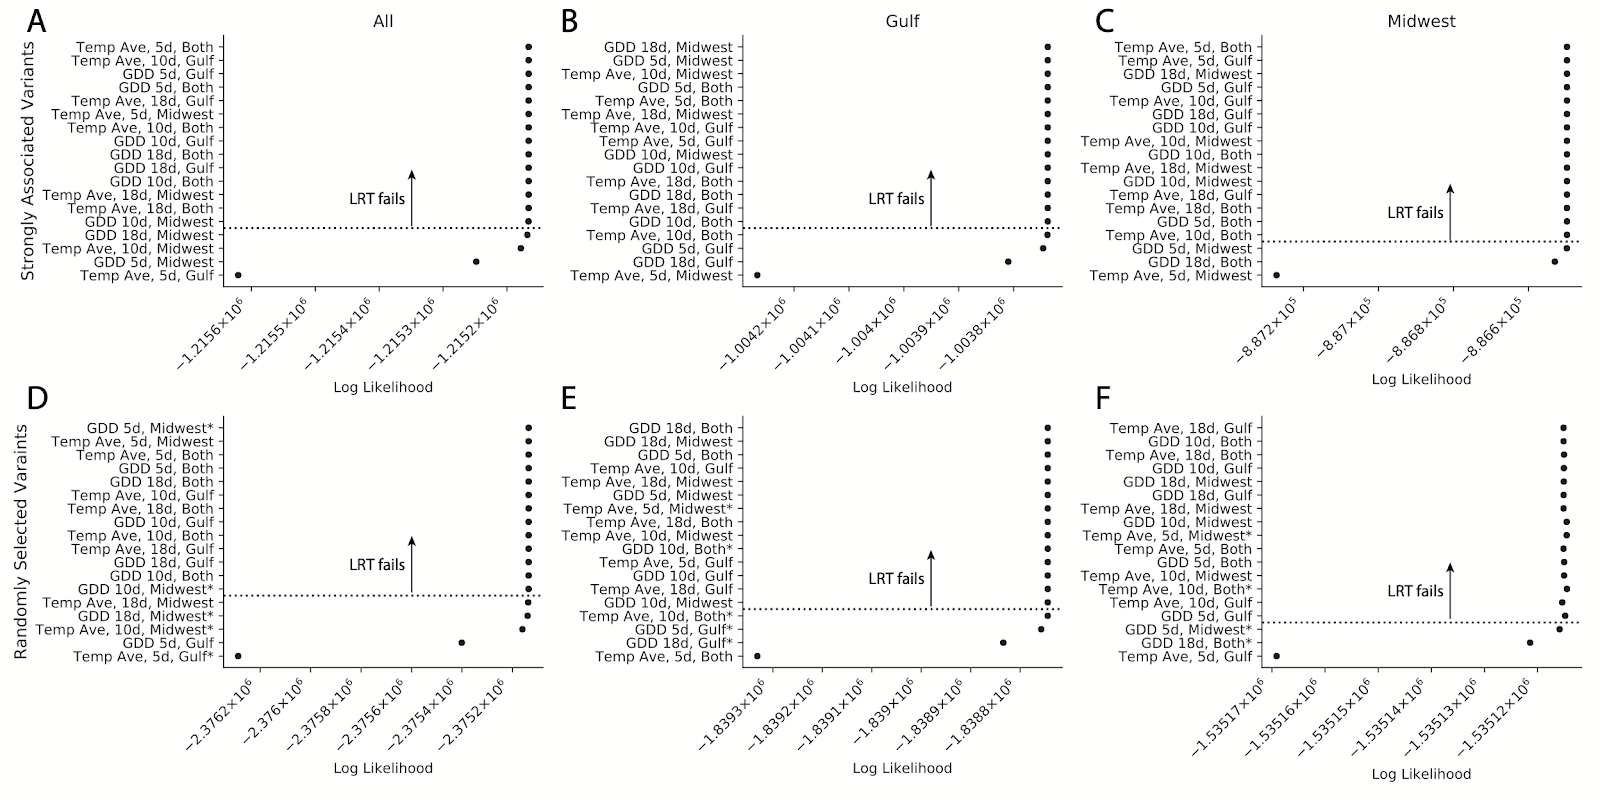
\includegraphics{images/RR_Figure1.png}

}

\caption{\textbf{Log-likelihood at each step in a greedy algorithm
implementation of model selection for mash for the green-up date
phenotype using only GxWeather covariance matrices.} The matrix that
resulted in the maximum likelihood model of covariance in summary
statistics among sites is located at the base of the y-axis; matrices
selected in the ensuing step are placed in ascending order along the
y-axis. (A) The maximum likelihood path of covariance matrices in the
greedy algorithm for the set of independent variants that were
significant in at least one context when analyzing all individuals. The
dashed black line represents the step in the algorithm where addition of
the next matrix did not significantly increase the model likelihood,
likelihood-ratio test p-value \textgreater{} 0.05. (B) and (C) show the
maximum likelihood paths when the individuals analyzed are only from the
Gulf and Midwest subpopulations, respectively. (D) The maximum
likelihood path of covariance matrices in the greedy algorithm for the
set of independent, randomly selected variants when analyzing all
individuals. The dashed black line represents the step in the algorithm
where addition of the next matrix did not significantly increase the
model likelihood, likelihood-ratio test p-value \textgreater{} 0.05. *
is used to denote those matrices that are identified by the greedy
algorithm in the set of significantly associated variants and the
randomly associated variants. (E) and (F) show the maximum likelihood
paths when the individuals analyzed are only from the Gulf and Midwest
subpopulations, respectively.}

\end{figure}%%
\begin{figure}[H]

{\centering 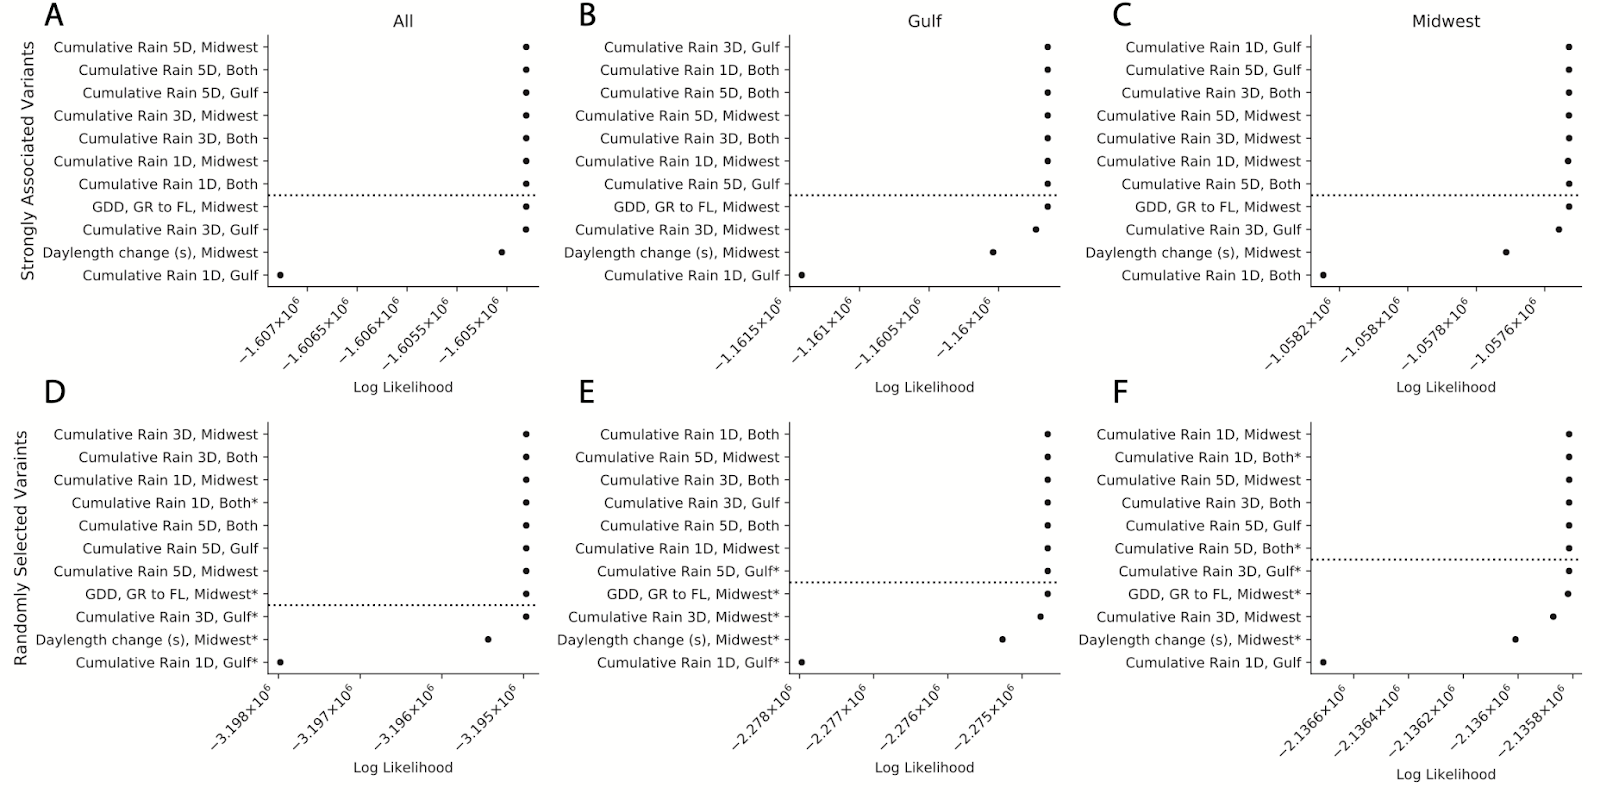
\includegraphics{images/RR_Figure2.png}

}

\caption{\textbf{Log-likelihood at each step in a greedy algorithm
implementation of model selection for mash for the flowering date
phenotype using only GxWeather covariance matrices.} The matrix that
resulted in the maximum likelihood model among sites is located at the
base of the y-axis; matrices selected in the ensuing step are placed in
ascending order along the y-axis. (A) The maximum likelihood path of
covariance matrices in the greedy algorithm for the set of independent
variants that were significant in at least one context when analyzing
all individuals. The dashed black line represents the step in the
algorithm where addition of the next matrix did not significantly
increase the model likelihood, likelihood-ratio test p-value
\textgreater{} 0.05. (B) and (C) show the maximum likelihood paths when
the individuals analyzed are only from the Gulf and Midwest
subpopulations, respectively. (D) The maximum likelihood path of
covariance matrices in the greedy algorithm for the set of independent,
randomly selected variants when analyzing all individuals. The dashed
black line represents the step in the algorithm where addition of the
next matrix did not significantly increase the model likelihood,
likelihood-ratio test p-value \textgreater{} 0.05. * is used to denote
those matrices that are identified by the greedy algorithm in the set of
significantly associated variants and the randomly associated variants.
(E) and (F) show the maximum likelihood paths when the individuals
analyzed are only from the Gulf and Midwest subpopulations,
respectively.}

\end{figure}%%
\begin{figure}[H]

{\centering 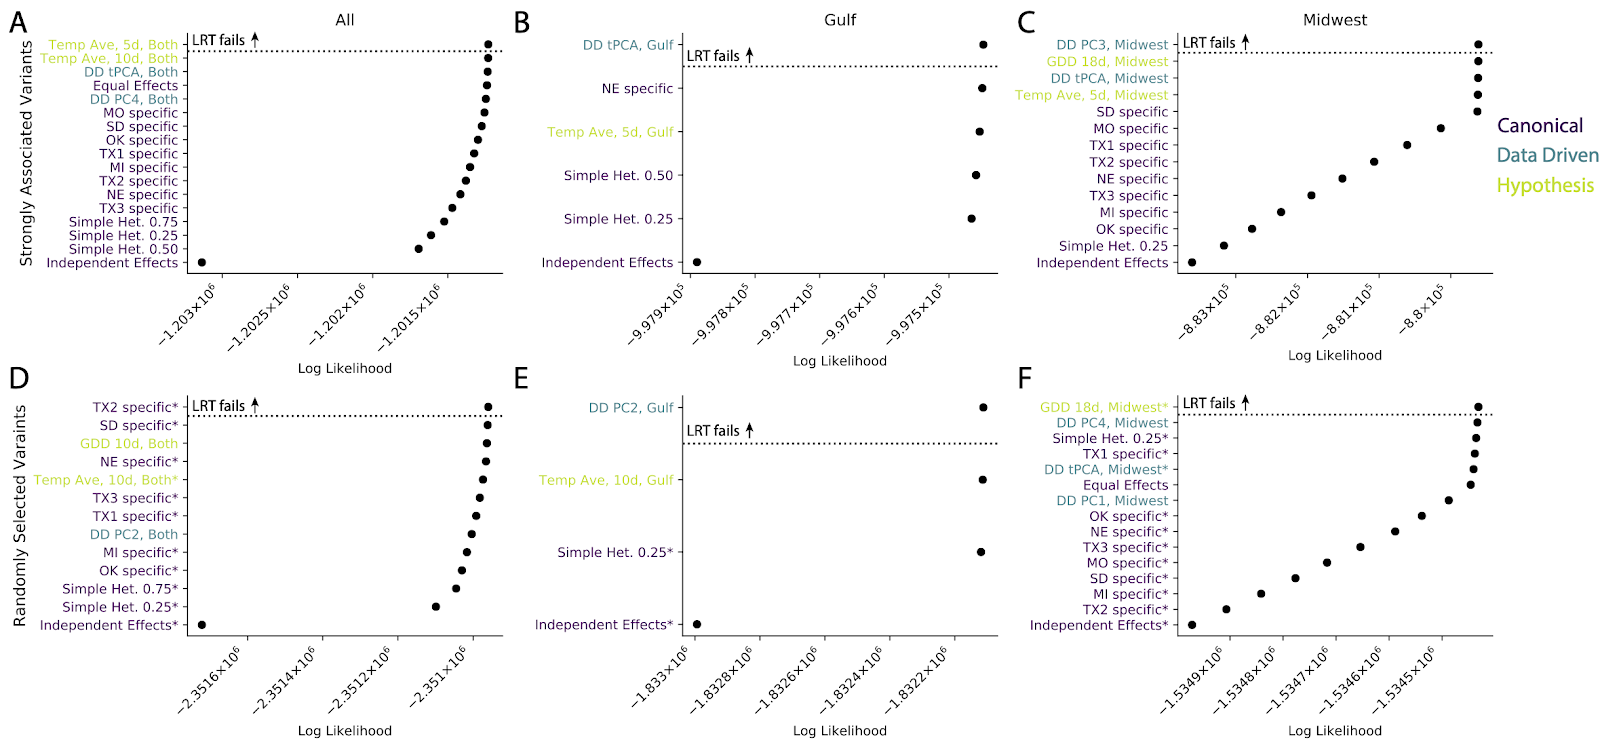
\includegraphics{images/RR_Figure3.png}

}

\caption{\textbf{Log-likelihood at each step in a greedy algorithm
implementation of model selection for mash for the greenup date
phenotype using canonical, data driven, and GxWeather covariance
matrices.} The matrix that resulted in the maximum likelihood model of
covariance in summary statistics among sites is located at the base of
the y-axis; matrices selected in the ensuing step are placed in
ascending order along the y-axis. (A) The maximum likelihood path of
covariance matrices in the greedy algorithm for the set of independent
variants that were significant in at least one context when analyzing
all individuals. The dashed black line represents the step in the
algorithm where addition of the next matrix did not significantly
increase the model likelihood, likelihood-ratio test p-value
\textgreater{} 0.05. Once this condition was met the greedy algorithm
was halted. (B) and (C) show the maximum likelihood paths when the
individuals analyzed are only from the Gulf and Midwest subpopulations,
respectively. (D) The maximum likelihood path of covariance matrices in
the greedy algorithm for the set of independent, randomly selected
variants when analyzing all individuals. The dashed black line
represents the step in the algorithm where addition of the next matrix
did not significantly increase the model likelihood, likelihood-ratio
test p-value \textgreater{} 0.05. Once this condition was met the greedy
algorithm was halted for computational considerations. * is used to
denote those matrices that are identified by the greedy algorithm in the
set of significantly associated variants and the randomly associated
variants. (E) and (F) show the maximum likelihood paths when the
individuals analyzed are only from the Gulf and Midwest subpopulations,
respectively.}

\end{figure}%%
\begin{figure}[H]

{\centering 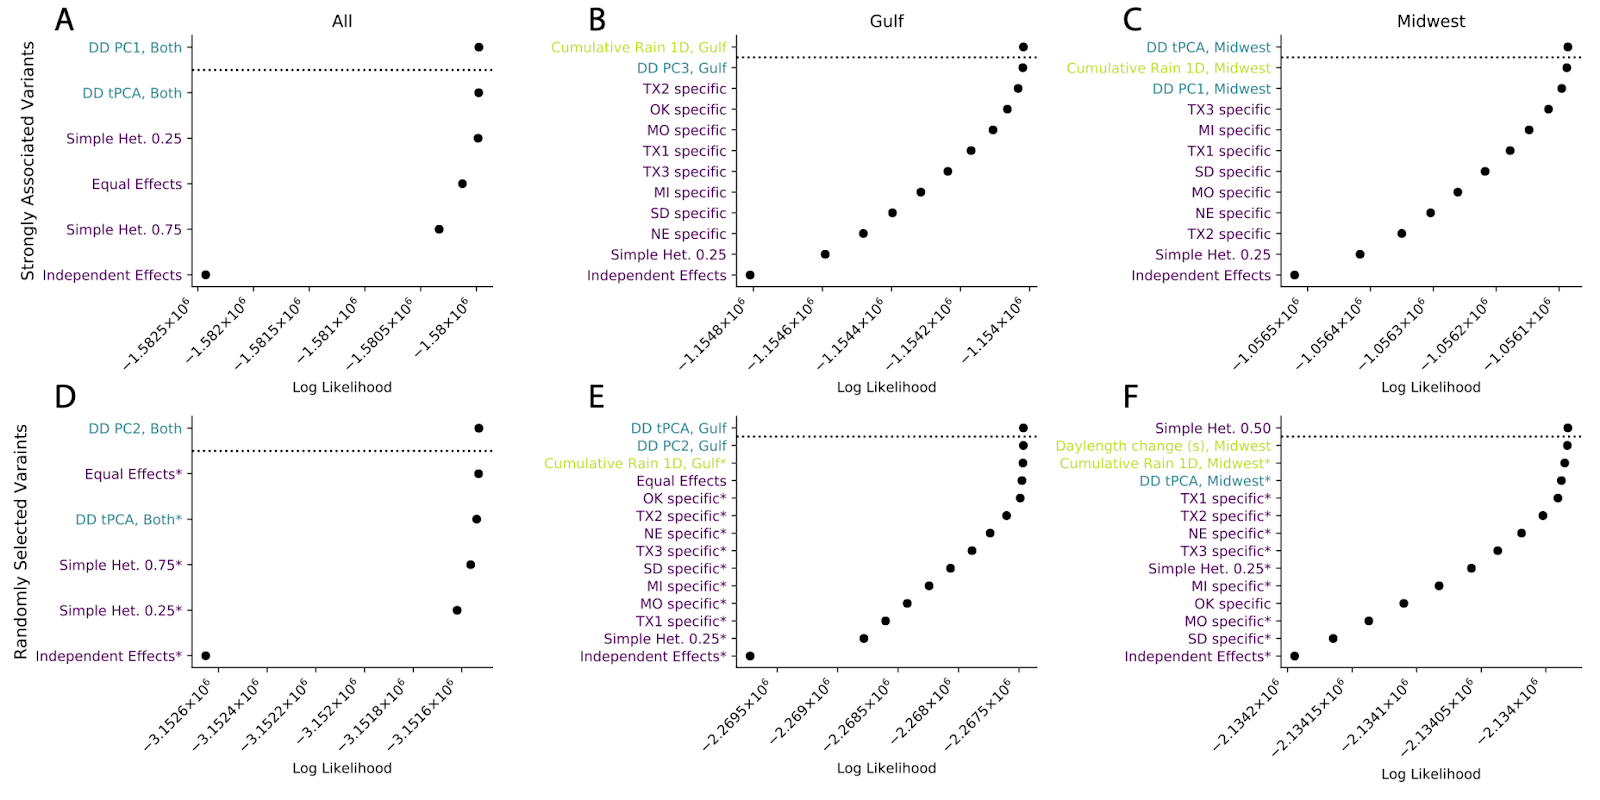
\includegraphics{images/RR_Figure4.png}

}

\caption{\textbf{Log-likelihood at each step in a greedy algorithm
implementation of model selection for mash for the flowering phenotype
using canonical, data driven, and GxWeather covariance matrices.} The
matrix that resulted in the maximum likelihood model of covariance in
summary statistics among sites is located at the base of the y-axis;
matrices selected in the ensuing step are placed in ascending order
along the y-axis. (A) The maximum likelihood path of covariance matrices
in the greedy algorithm for the set of independent variants that were
significant in at least one context when analyzing all individuals. The
dashed black line represents the step in the algorithm where addition of
the next matrix did not significantly increase the model likelihood,
likelihood-ratio test p-value \textgreater{} 0.05. Once this condition
was met the greedy algorithm was halted. (B) and (C) show the maximum
likelihood paths when the individuals analyzed are only from the Gulf
and Midwest subpopulations, respectively. (D) The maximum likelihood
path of covariance matrices in the greedy algorithm for the set of
independent, randomly selected variants when analyzing all individuals.
The dashed black line represents the step in the algorithm where
addition of the next matrix did not significantly increase the model
likelihood, likelihood-ratio test p-value \textgreater{} 0.05. Once this
condition was met the greedy algorithm was halted for computational
considerations. * is used to denote those matrices that are identified
by the greedy algorithm in the set of significantly associated variants
and the randomly associated variants. (E) and (F) show the maximum
likelihood paths when the individuals analyzed are only from the Gulf
and Midwest subpopulations, respectively.}

\end{figure}%

\begin{quote}
\begin{tcolorbox}[enhanced jigsaw, rightrule=.15mm, colframe=quarto-callout-warning-color-frame, leftrule=.75mm, arc=.35mm, colback=white, opacityback=0, left=2mm, breakable, toprule=.15mm, bottomrule=.15mm]

- There appears to be an issue with the construction of the
hypothesis-derived covariance matrices. I believe the goal here is to
estimate the genetic covariance among gardens based on the phenotypic
covariance (P) and the estimated residual covariance (E), where P = G +
E. The described approach involves starting with the the phenotypic
correlation matrix and then replacing the diagonal with the coefficient
of variation. If the diagonal had been replaced with the h2 in each
garden, that'd be a valid estimate of G. But as described, it's likely
that you'll end up with an invalid covariance matrix, one that's not
positive-semi-definite. Instead the appropriate operation would be to
both pre- and post-multiply the covariance matrix by a diagonal matrix
with the square-root of the CV's. This maintains a valid covariance-like
structure. Or just mean-standardize the traits first and then calculate
the covariance of this standardized matrix.

\end{tcolorbox}
\end{quote}

We now use the narrow-sense heritability as the diagonal for each
GxWeather matrix, and clarify this in the Supplementary Methods (SI
Appendix, Section S1, first and eighth paragraph - first and last
paragraph on page two).

\begin{quote}
\begin{tcolorbox}[enhanced jigsaw, rightrule=.15mm, colframe=quarto-callout-warning-color-frame, leftrule=.75mm, arc=.35mm, colback=white, opacityback=0, left=2mm, breakable, toprule=.15mm, bottomrule=.15mm]

- Antagonistic Pleiotropy: Maybe I'm missing the idea of this analysis,
but it doesn't seem to me that this strategy for partitioning loci
between antagonistic pleiotropy and differential sensitivity would have
equal power to detect each class. It seems that antagonistic pleiotropy
should be a subset of differential sensitivity because the latter is
defined as simply a change in magnitude. But even if it's restricted to
``different magnitude but same sign'', the practical definition here
seems to be that antagonistic pleiotropy is detected when the signs are
different and both lfsrs \textless{} threshold (0.05?), while
differential sensitivity additionally requires a threshold on the
difference in effect sizes (0.4) with no justification for why this size
was chosen. This additional criterion will necessarily make the rate of
detection different. Even without this, with differential sensitivity
one effect size must be much larger than the other in absolute value
(which isn't the case with antagonistic pleiotropy), so differential
sensitivity loci will be more likely to pass the lfsr loci than
antagonistic pleiotropy loci. Note that previous literature here tried
to separate antagonistic pleiotropy from conditional neutrality (ie
where in one location the effect was zero), while here the contrast is
with differential sensitivity where effects are non-zero in all
locations. I'm not aware of previous discussions in the literature of
trying to differentiate these two specific classes of GxE variants and
not really sure theoretically what the importance would be.

\end{tcolorbox}
\end{quote}

We believe that the use of the lfsr to detect effects with rank-changing
GxE is a key advance in our manuscript, and so we have made changes to
the Introduction (lines 175-177), Results (lines 338-343), and Materials
\& Methods (lines 959-982; lines 996-998; lines 1055-1057) to explain
and motivate this statistical change.

Our expectation is that in nature, effects will always differ.
Statistically, this difference will not always be detectable. Thus,
rather than ask ``Are these two effects different?'' - as we reasonably
expect two effects to be, even if this difference cannot be measured -
the local false sign rate answers a more meaningful question: Can we be
confident in the sign of this effect?

We think that if evolutionary geneticists are interested in antagonistic
pleiotropy and rank-changing GxE, then they should use the lfsr to
measure their confidence in the sign of the effect, rather than using
statistical tests where the null hypothesis is that the effect is
different than zero. However, if we use the lfsr, comparisons between
antagonistic pleiotropy and conditional neutrality are no longer
sensible, as we are no longer doing a statistical test that can robustly
detect conditional neutrality (just as the FDR does not robustly detect
antagonistic pleiotropy). This is justified because detection of
antagonistic pleiotropy is more important than detection of conditional
neutrality for models of local adaptation.

It's true that the threshold for differential sensitivity is arbitrary.
We have reworded the manuscript to stress that there is equal power to
detect effects of different sign as there are effects of the same sign
(lines 996-998; lines 1055-1057). Another class of effects we have in
our analysis that differ from classic antagonistic pleiotropy \&
conditional neutrality comparisons are effects which are not
distinguishable by sign or magnitude. It is not accurate that
differentially sensitive loci will be more likely to pass the lfsr,
because the loci are first selected by significant lfsr, then divided
further into effects that can \& cannot be distinguished by magnitude.
Thus effects that are significant, but have small magnitude in both
conditions will be labeled as not being distinguishable - essentially,
these effects do not have detectable GxE. Effects without GxE may be
even more common and should also be quantified. We propose that, if our
intent is to detect sign-changing GxE, then we should use an unbiased
statistical test to look at loci with and without sign-changing GxE, the
lfsr.

~

~

\begin{center}
Best,

\end{center}

\begin{flushright}
Alice MacQueen and Tom Juenger

\end{flushright}



\end{document}
